% Chapter Template

\chapter{Avaluació del sistema} % Main chapter title

\label{Chapter8} % Change X to a consecutive number; for referencing this chapter elsewhere, use \ref{ChapterX}

Tot projecte ha d'estar validat i avaluat per un conjunt de directrius concretes per contemplar el projecte com a finalitzat. En aquest capítol s'explicarà com s'han realitzat aquestes proves i quines eines s'han utilitzat. Les proves s'han realitzat durant el desenvolupament i la fase final d'aquest, quan ja el producte pràcticament es podia donar per finalitzat.

%----------------------------------------------------------------------------------------
% SECTION 1
%----------------------------------------------------------------------------------------

\section{Proves durant el desenvolupament}

Com s'ha comentat en el capítol anterior, s'ha tingut molta cura en l'enregistrament de versions de l'aplicació. Quan un conjunt d'històries d'usuari es considerava implementat, es versionava aquella part del codi i es marcava constància en el repositori.
\\\\
Durant el desenvolupament de les funcionalitats sempre es provava el funcionament d'aquestes fins que es complissin tots els criteris d'acceptació de la història d'usuari corresponent. Tot i així, el fet que un sol usuari proves aquell conjunt de funcionalitats no es va considerar suficient per validar si aquella versió del codi era funcional amb els requisits especificats.
\\\\
Partint d'aquest aspecte, es va decidir utilitzar les funcionalitats de les quals disposa \textit{Google Play} per penjar versions d'aplicacions alfa i/o beta. Són versions que no són públiques de cara al públic però que si pots retransmetre a un conjunt d'usuaris concret. Es va decidir demanar el favor a un seguit d'estudiants de la facultat, als quals se'ls demanava la prova de les funcionalitats concretes d'aquella versió. S'especificava que prestessin atenció en els moviments que realitzaven i com era la interacció amb la plataforma. Un cop es provava l'aplicació, es realitzava una retrospectiva amb cadascun d'ells per veure quins aspectes havien trobat positius i quins mancaven en el flux de l'aplicació.
\\\\
Per a poder seguir aquest procediment més pròximament es va decidir utilitzar les funcionalitats que et permetia \textit{Firebase}. Ja que, a més de ser una base de dades com s'ha comentat anteriorment, disposa d'un conjunt d'eines que et permet saber les estadístiques de l'aplicació i, en cas de fallida, quina traça d'error havia generat dita fallida. Així doncs, quan hi havia una fallida en el transcurs de l'aplicació aquesta era notificada a \textit{Firebase} i aquest captava tota la informació d'error. Informació com la mateixa traça d'error però també el model del mòbil utilitzat, la versió d'Android, el percentatge de bateria en aquell precís moment i més detalls per a poder identificar de la forma més fàcil possible el motiu d'aquella fallida.
\\
\begin{figure}[H]
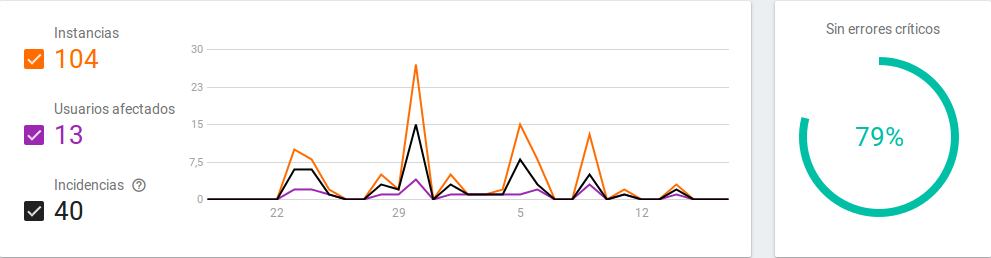
\includegraphics[scale=0.405]{Figures/crash_analytics.png}
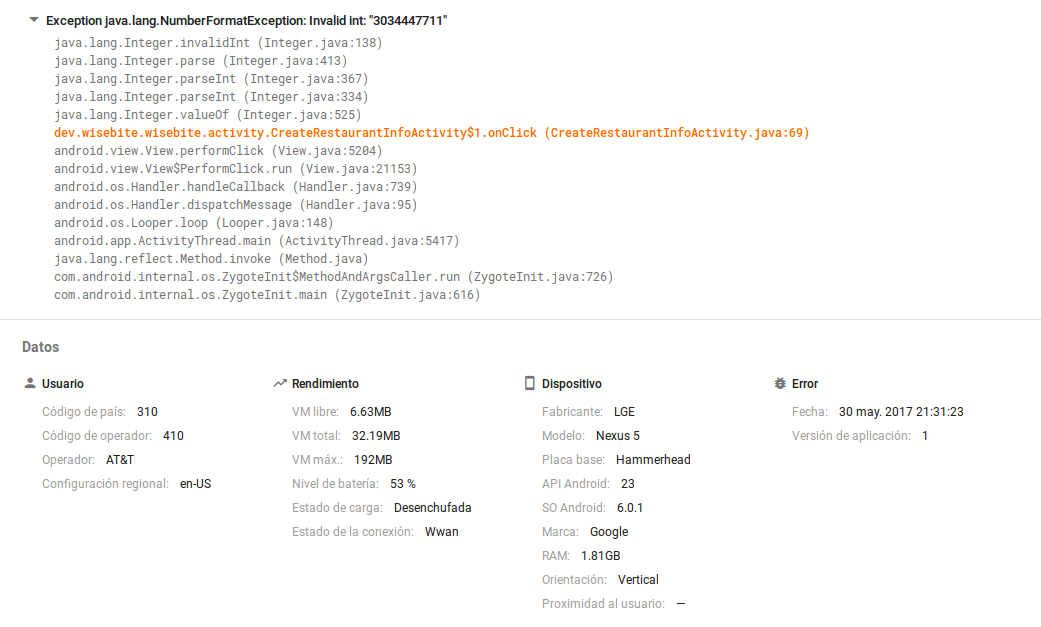
\includegraphics[scale=0.385]{Figures/crash.png}
\caption{Estadístiques d'errors proporcionades per Firebase}
\end{figure}

\noindent I així es va arribar fins a la versió \textit{1.0} de la plataforma. Un cop arribats a aquest punt l'aplicació va ser desplegada de forma definitiva al \textit{Google Play} i va ser publica a tot el món.

%----------------------------------------------------------------------------------------
% SECTION 2
%----------------------------------------------------------------------------------------

\section{Proves finals}

Un cop l'aplicació va formar part de la galeria d'aplicacions de \textit{Google Play}, es va decidir emfatitzar les proves a un conjunt d'usuaris que no fossin de la branca d'informàtics, sinó possibles usuaris de l'aplicació en un mercat real. Es va contactar amb coneguts del sector de la restauració perquè es descarreguessin l'aplicació i la provessin. A aquests usuaris no se'ls va donar cap tipus de formació ni d'aprenentatge previ, ja que es volia estudiar com era d'intuïtiva \textit{Wisebite}.
\\\\
Després de dues setmanes de proves amb aquests usuaris, els quals van acabar convertint-se en un conjunt de 26 persones, es van versionar dues vegades més fins a la versió \textit{1.2} de l'aplicació. Durant aquesta evolució del codi es va escoltar la seva veu i es va implementar les millores que es veien necessàries per \textit{Wisebite}.